\label{Komponenten}

Das Komponentendiagramm, welches in \ref{fig:KomponentenDiagramm} zu sehen ist, soll dazu dienen, alle Aktoren und deren Verbindungen darzustellen. \\
So teilten wir den Arduino als Controll-Hardware in drei Komponenten. Die Profilauswahl importiert drei Eingangssignale, welche bei Betätigung der Taster, gesendet werden. Je nach Menü sind diese Signale unterschiedlich zu interpretieren. Zudem werden die übersetzten Botschaften, je nach Fall, an das \ac{LCD}-Display oder die Messeinrichtung weitergeleitet. \\
Der CO$_2$-Sensor sendet ausschließlich nach Aufforderung der Messeinrichtung den gemessenen CO$_2$-Wert, welcher an die Mikro-SD-Karte und die CO$_2$-Auswertung weitergeleitet wird. In der Mikro-SD werden die Daten abgespeichert, während die Auswertung der Messwerte die unterschiedlichen \ac{LED}s ansteuert.

\begin{figure}[!hbt]
	\centering
	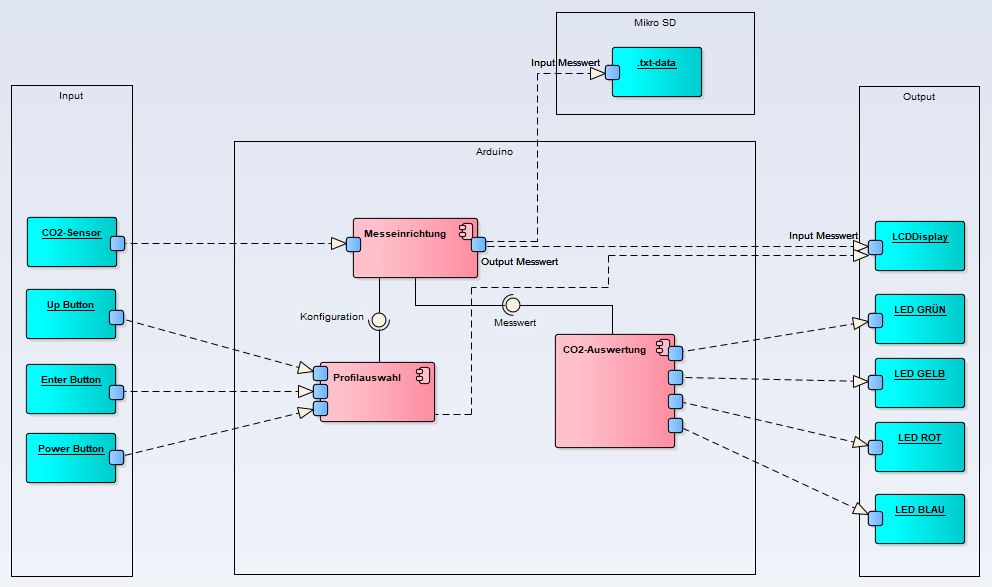
\includegraphics[width=0.9\linewidth]{Images/Komponentendiagramm}
	\caption{Entwurf des Komponentendiagramms mithilfe von Enterprise Architect}
	\label{fig:KomponentenDiagramm}
\end{figure}